\begin{figure}[p]
\centering
\captionsetup{justification=raggedright,labelsep=none,singlelinecheck=false,labelformat=boldlabel}
\caption[Out-of-sample RMSE gains relative to HAR.]{\footnotesize \textbf{: Out-of-sample RMSE gains relative to HAR.} Pooled-panel and factor-only results take the square root after pooling squared errors across all available target-month observations. They are not averages of factor-level RMSE. The two market-portfolio results evaluate a single monthly series. Positive values indicate lower RMSE than HAR.}
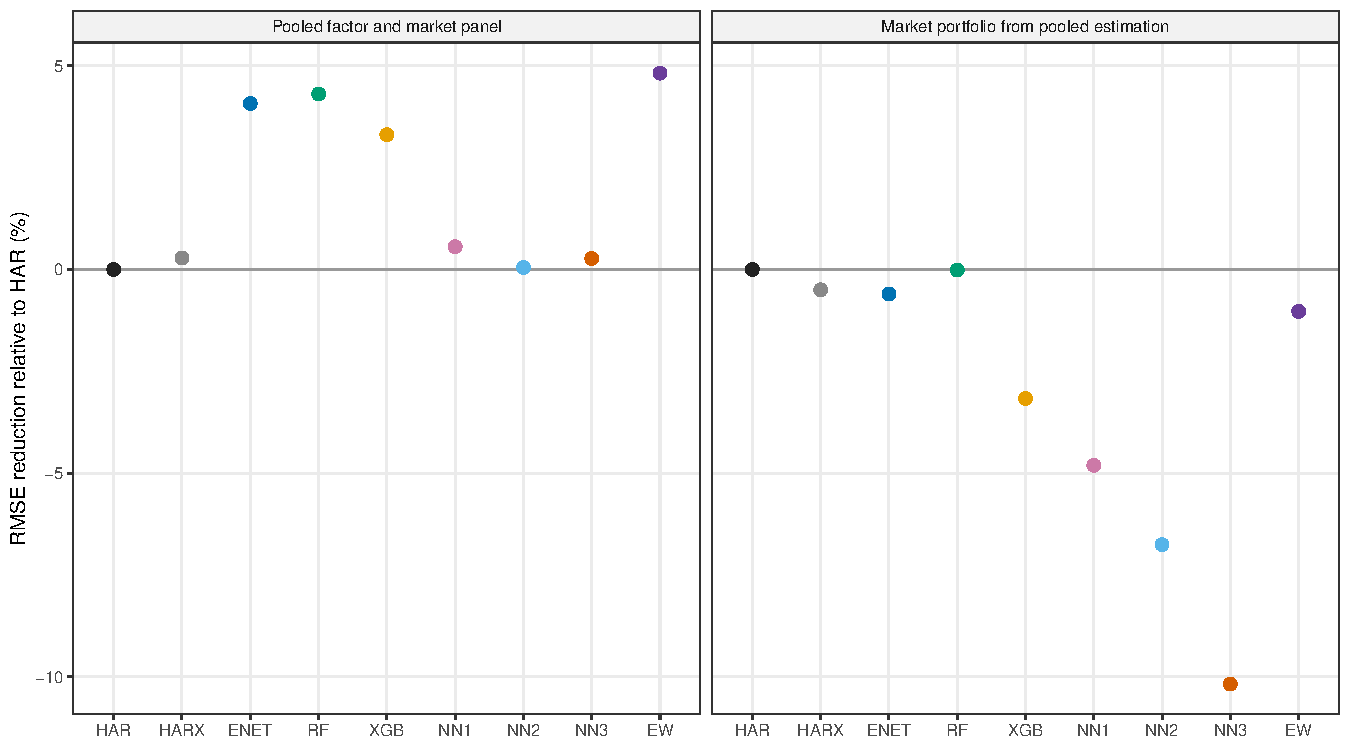
\includegraphics[width=\linewidth,height=0.78\textheight,keepaspectratio]{results_v3/1986/main/har_relative_gains.pdf}
\label{fig:rv-har_relative_gains}
\end{figure}
